\section{Evaluation}
\label{sec:evaluation}
We implement (\S\ref{sec:implementation}) and evaluate \sysname and evaluate across
five metrics: \textbf{Forward Latency} (\S~\ref{subsec:forward-latency}),
\textbf{GPU Utilization} (\S~\ref{subsec:gpu-utilization}),
\textbf{Overlap Efficiency} (\S~\ref{subsec:overlap-efficiency}),
\textbf{Throughput} (\S~\ref{subsec:throughput}), and \textbf{Expert Scalability} (\S~\ref{subsec:expert-scalability}).
We run experiments on a server with 8 NVIDIA H100 80G GPUs interconnected via NVLink,
125 GB of RAM, and 20 vCPUs. We used PyTorch 2.6.0, CUDA 12.8, and Ubuntu 22.04.
All experiments use MoE transformer models configured with 16 attention heads,
an embedding dimension of 2048, and an FFN intermediate size of 2048.
We apply Distributed Data Parallelism (DDP) and Expert Parallelism for all experiments.
We execute only the forward pass over a single MoE layer and measure the average runtime
of 32 passes after 32 warmup passes.
We use top-2 routing with a capacity factor of 1.0.
We compare \sysname against several state-of-the-art MoE systems:
(1) \textbf{Comet}~\cite{comet}, 
(2) \textbf{FasterMoE}~\cite{fastermoe}, 
(3) \textbf{Megatron-CUTLASS}~\cite{megatron-lm}, and
(4) \textbf{Megatron-TE}: Megatron-LM with Transformer Engine~\cite{transformer-engine}.
Comet relies on~\verb|cudaMemcpyPeerAsync|~\cite{fluxp2p}, while FasterMoE and Megatron-LM use NCCL exclusively for communication.
%We also evaluate \sysname on a multi-node environment and discuss our findings in \S\ref{sec:multi-node-evaluation}.

\myparab{Desiderata}.
We observe Comet exhibiting anomalously bad performance values at 8 GPUs,
so we exclude their results from evaluations at 8 GPUs and only include for results at $\leq$
4 GPUs. We evaluate \sysname using FP32 precision whereas all baselines use FP16.
We do so because (1) of incomplete fp16 tuning (\S\ref{sec:fp16-memory-throughput})
and (2) no baseline supports FP32.
Note, this precision discrepancy disadvantages \sysname by doubling its
communication volume and computational workload.
\subsection{Forward Latency}\label{subsec:forward-latency}
\begin{figure}[!h]
    \centering
    \begin{subfigure}{0.49\textwidth}
        \centering
        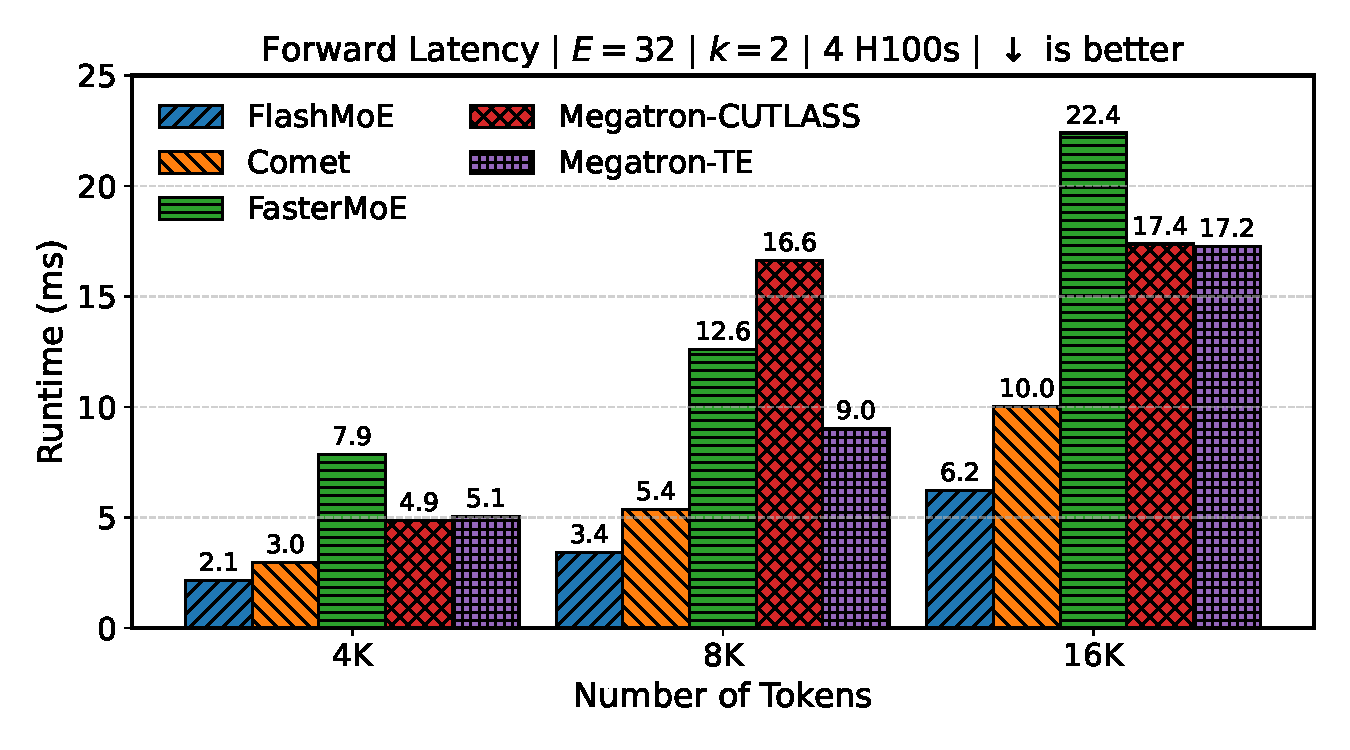
\includegraphics[width=\linewidth, keepaspectratio]{flash_figs/scaling_tokens}
        \caption{4 H100s}
        \label{sub:4gl}
    \end{subfigure}
    \begin{subfigure}{0.49\textwidth}
        \centering
        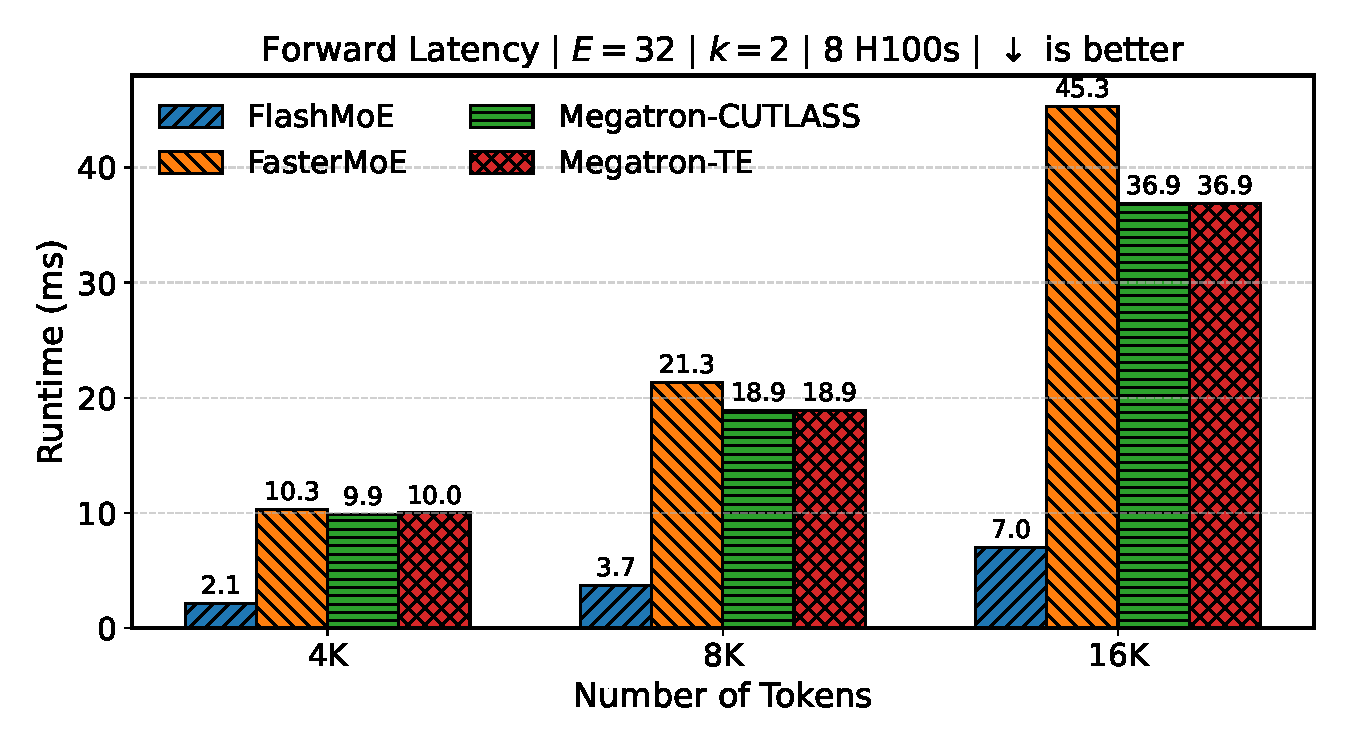
\includegraphics[width=\linewidth, keepaspectratio]{flash_figs/scaling_tokens_8}
        \caption{8 H100s}
        \label{sub:8gl}
    \end{subfigure}
    \caption{Forward Latency as the \emph{Number of Tokens} per GPU increases.}
    \label{fig:fl}
\end{figure}
We first measure the forward latency of FlashDMoE across different sequence lengths on both 4 and 8 GPU setups
(Figure~\ref{fig:fl}).
FlashDMoE consistently outperforms all baselines,
with especially notable improvements at longer sequence lengths.
On 4 GPUs, it achieves up to \textbf{4.6}x speedup over Megatron-TE at 16K tokens,
and \textbf{2.6}x over FasterMoE.
The gains are even more pronounced at 8 GPUs
where FlashDMoE maintains low latency, exhibiting up to \textbf{6.4}x speedup over baselines that
degrade steeply due to increasing communication costs as token buffers increase proportionally.
%These results highlight FlashDMoE’s ability to scale token throughput without suffering from the communication
%penalties that plague other implementations.
\subsection{GPU Utilization}\label{subsec:gpu-utilization}
\begin{wrapfigure}{r}{0.5\textwidth}
    \vspace{-10pt}
    \centering
    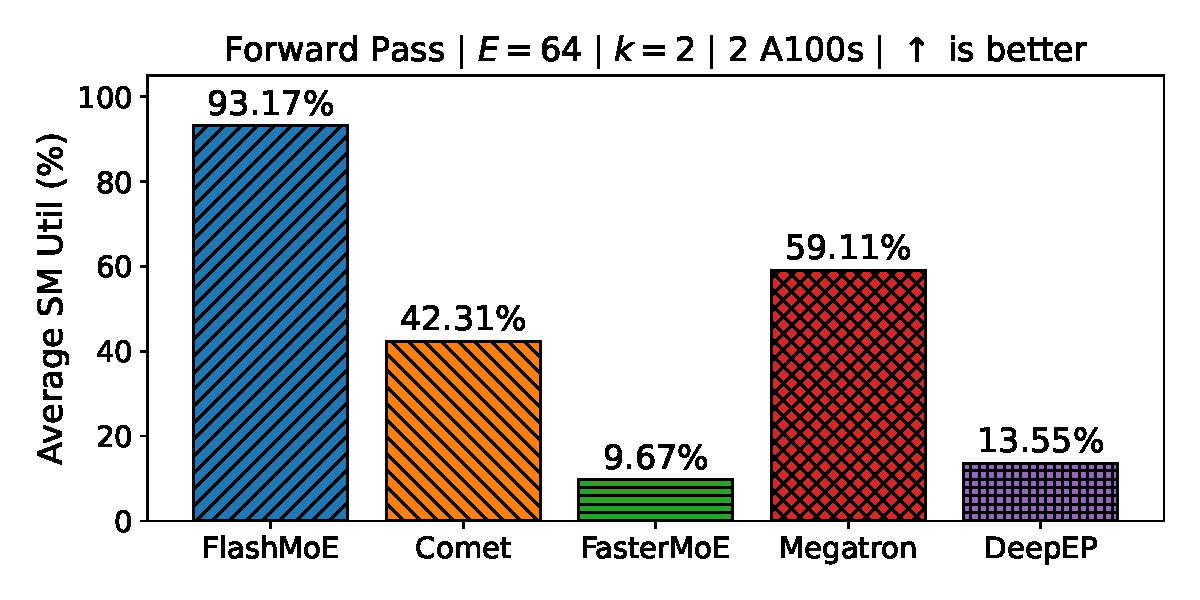
\includegraphics[width=0.9\linewidth, keepaspectratio]{flash_figs/sm_util}
    \caption{SM utilization, defined as the ratio of cycles in which SMs
    have at least one warp in flight
    to the total number of cycles~\cite{nsight-metrics}.
    Values represent the average SM utilization over 100 iterations.}
    \label{fig:smu}
\end{wrapfigure}
To quantify GPU efficiency, we measure Streaming Multiprocessor (SM) utilization during the forward pass (Figure~\ref{fig:smu}).
FlashDMoE achieves 93.17\% average SM utilization,
over \textbf{9}x higher than FasterMoE (9.67\%), \textbf{6.8}x higher than DeepEP+Megatron-LM (13.55\%)
\textbf{4}x higher than Megatron-TE (59.11\%), and
\textbf{2.2}x higher than Comet (42.31\%).
This improvement stems from our fully fused kernel architecture and
fine-grained pipelining of compute and communication tasks.
By eliminating idle gaps due to kernel launches and enabling in-kernel task scheduling,
FlashDMoE ensures SMs remain busy with productive work throughout execution.

\subsection{Overlap Efficiency}\label{subsec:overlap-efficiency}
\begin{figure}[!h]
    \centering
    \begin{subfigure}{0.49\textwidth}
        \centering
        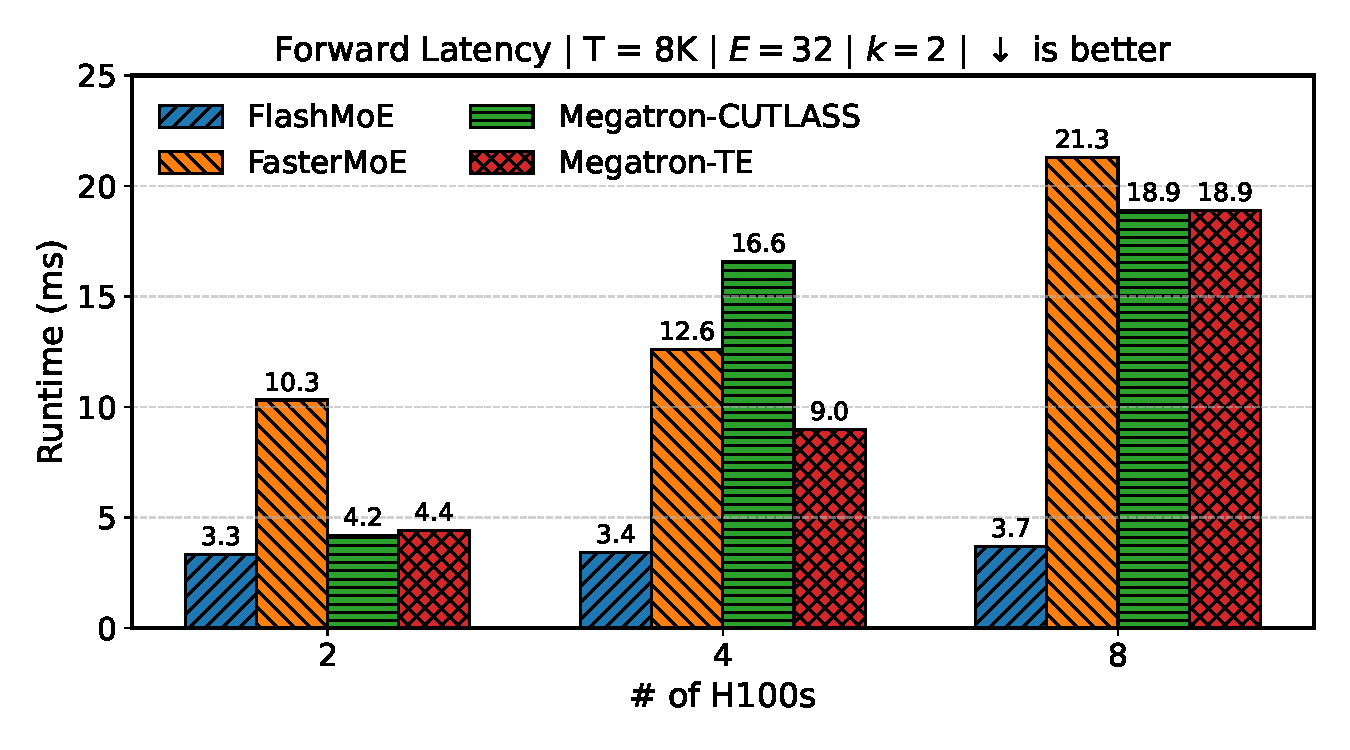
\includegraphics[width=\linewidth, keepaspectratio]{flash_figs/scaling_gpus_8}
        \caption{Latency as Number of GPUs increases.}
        \label{fig:lng}
    \end{subfigure}
    \begin{subfigure}{0.49\textwidth}
        \centering
        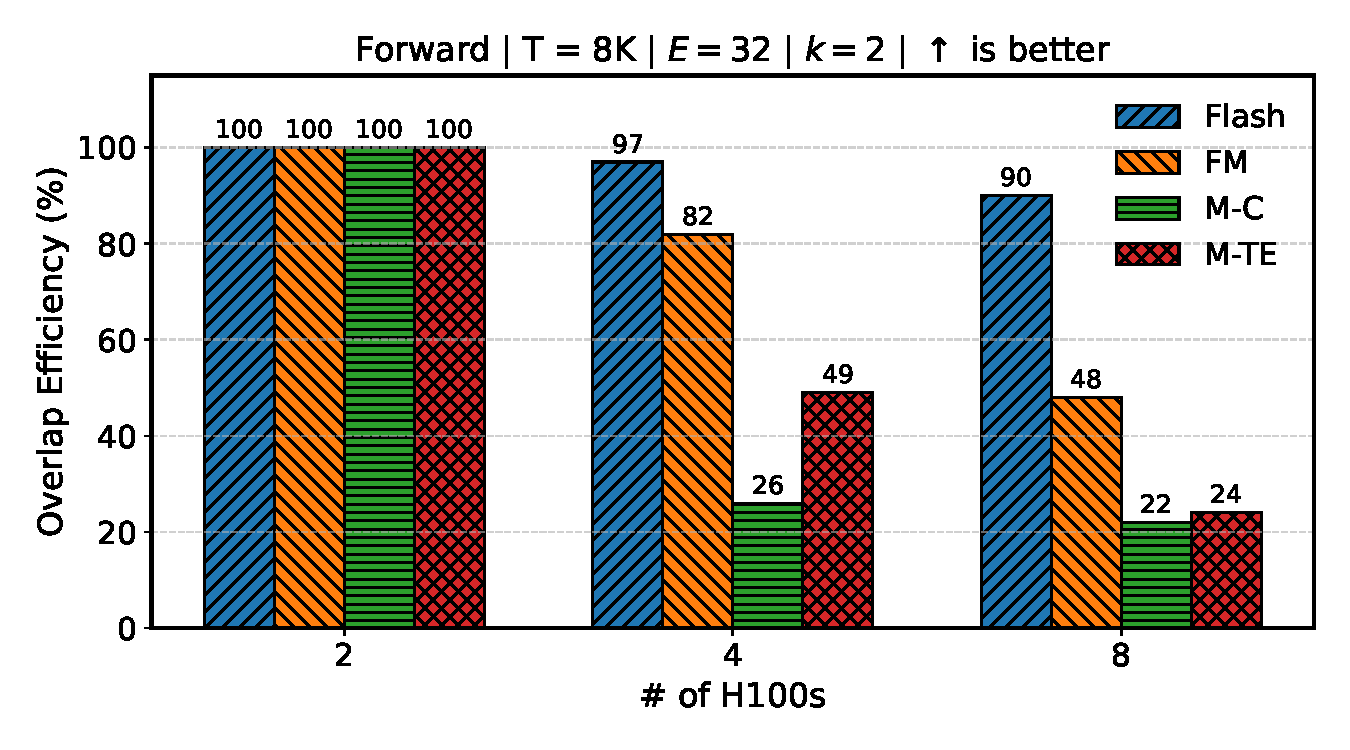
\includegraphics[width=\linewidth, keepaspectratio]{flash_figs/overlap_efficiency_8}
        \caption{Weak scaling efficiency}
        \label{fig:oe}
    \end{subfigure}
    \caption{Forward Latency as the \emph{Number of Tokens} per GPU increases. We define Overlap Efficiency $O_e$
        to be $O_e = T(2) / T(N_G)$, where $T(N_G)$ is the latency at $N_G$ GPUs and $T(2)$ is the latency at 2 GPUs.}
    \label{fig:oet}
\end{figure}
We evaluate the extent to which \sysname overlaps communication and computation by measuring weak scaling efficiency
as the number of GPUs increases (Figure~\ref{fig:oe}).
We note that most baselines fail to execute at a single GPU, hence why we use 2 GPUs as the reference point.
We observe that Megatron-CUTLASS and Megatron-TE degrade significantly,
with overlap efficiency dropping below 50\% at $\geq 4$ GPUs. \sysname gives up to \textbf{3.88}x and
\textbf{4}x higher efficiency at 4 and 8 GPUs, respectively.
Figure~\ref{fig:lng} further illuminates this efficiency, as \sysname shows stable forward latency growth.
These results corroborate that \sysname's actor-based design and asynchronous data movement
achieve near-ideal overlap.
%whereas baselines Megatron-CUTLASS and Megatron-TE experience approximately linear
%latency amplification while FasterMoE exhibits sublinear scaling.
%We attribute this suboptimal performance to exposed communication.
%In contrast, \sysname demonstrates uniform latency as expected since the workload per
%GPU is fixed in this weak scaling experiment.
%These results corroborate that \sysname's actor-based design and asynchronous data movement
%achieve near-ideal overlap.
\subsection{Throughput}\label{subsec:throughput}
\begin{wrapfigure}{r}{0.4\textwidth}
    \vspace{-15pt}
    \centering
    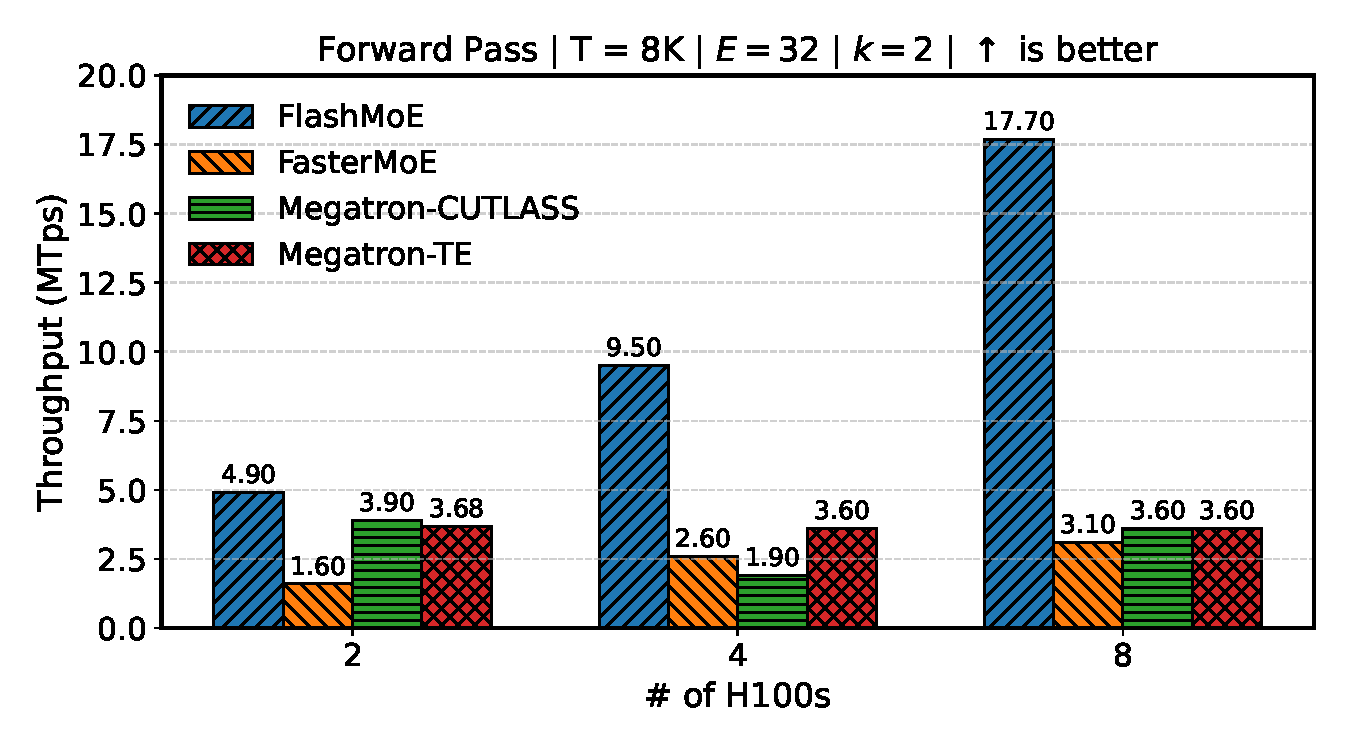
\includegraphics[width=0.9\linewidth, keepaspectratio]{flash_figs/throughput_8}
    % \caption{Throughput as the amount of GPUs increases. We compute throughput as $\frac{T * N_G}{latency}$, where $N_G$ is the number of GPUs.}
    \caption{Throughput when scaling the number of GPUs, computed as $\frac{T \times N_G}{\text{latency}}$.}
    \label{fig:thr}
\end{wrapfigure}
As shown in Figure~\ref{fig:thr}, \sysname scales linearly with GPU count, reaching 17.7 MTokens/s at 8 GPUs.
This is over \textbf{5.7}x higher than FasterMoE and \textbf{4.9}x higher than Megatron-TE and Megatron-CUTLASS\@.
Notably, these results are achieved despite \emph{FlashDMoE operating entirely in FP32,
while baselines use FP16}.
This indicates that FlashDMoE’s design eliminates throughput bottlenecks not by
exploiting lower precision, but by maximizing hardware utilization and eliminating host-driven inefficiencies.
\subsection{Expert Scalability}\label{subsec:expert-scalability}
\begin{figure}[!h]
    \centering
    \begin{subfigure}{0.49\textwidth}
        \centering
        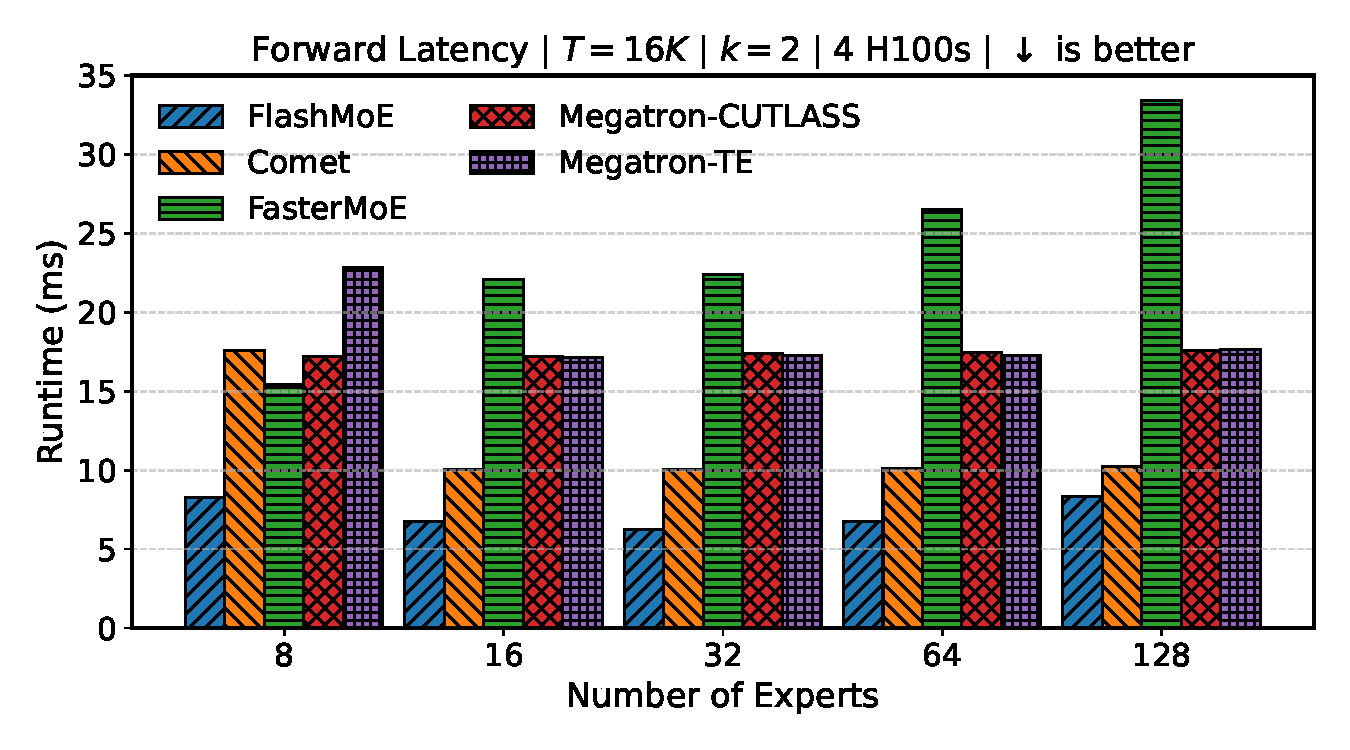
\includegraphics[width=\linewidth, keepaspectratio]{flash_figs/scaling_experts}
        \caption{4 H100s}
        \label{sub:4gx}
    \end{subfigure}
    \begin{subfigure}{0.49\textwidth}
        \centering
        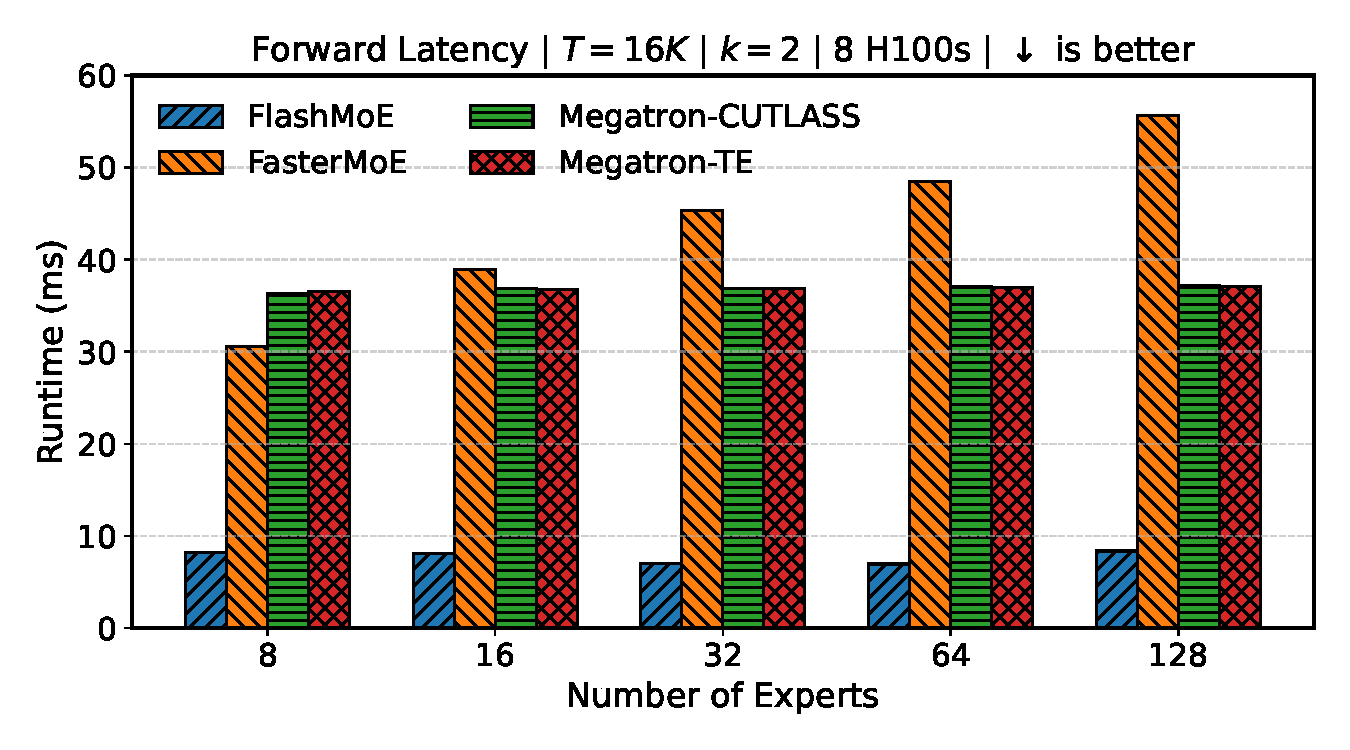
\includegraphics[width=\linewidth, keepaspectratio]{flash_figs/scaling_experts_8}
        \caption{8 H100s}
        \label{sub:8gx}
    \end{subfigure}
    \caption{Forward Latency as the \emph{Number of experts} increases.}
    \label{fig:xs}
\end{figure}
We analyze how \sysname scales with increasing number of experts at fixed sequence length (T = 16K).
Note that for the discussed plots, the number of experts on the x-axis is the \emph{total number across all GPUs}.
Each GPU gets 1/8th of this value.
As seen in Figure\ref{fig:xs}, \sysname maintains \emph{low, uniform} latency, as desired,
even as the number of experts grows from 8 to 128.
In contrast, baselines exhibit superlinear latency increases due to increased kernel launch overheads.
\sysname outperforms these baselines by up to \textbf{4}X at 4 H100s and \textbf{6.6}X at 8 H100s, both at 128 experts.
\sysname’s payload-efficient communication and scheduler-driven
in-kernel dispatching allow it to sustain expert parallelism
without incurring the communication and orchestration penalties seen in other systems.
These results reinforce FlashDMoE’s scalability for ultra-sparse MoE configurations.
